\documentclass[portrait,a0,oldgerm]{a0poster}
\usepackage{ascmac}
\usepackage{amsmath}
\usepackage{bm}
\usepackage{bnf}
\usepackage[dvips]{graphicx,epsfig}
\usepackage{xcolor,lipsum}
\usepackage{multicol}
\usepackage{multirow}
%\usepackage{ulem}
%\usepackage{udline_euc}
\usepackage{wallpaper}
\setlength{\columnsep}{50pt}
\setlength{\fboxrule}{3pt}
\pagestyle{empty}
\def\thesection{\fontsize{46}{20}\selectfont \Roman{section}.}
\def\thesubsection{\fontsize{46}{20}\selectfont \roman{subsection}.}
\def\thesubsubsection{\fontsize{46}{20}\selectfont \roman{subsection}.\roman{subsubsection}.}
\def\baselinestretch{1.07}
\def\formularsize{\fontsize{60}{20}\selectfont}
\def\normalfontsize{\fontsize{36}{20}\selectfont}
\def\spaceV{\ \ \ \ \ }
\def\spaceX{\ \ \ \ \ \ \ \ \ \ }
\def\spaceXV{\ \ \ \ \ \ \ \ \ \ \ \ \ \ \ }
\def\spaceXX{\ \ \ \ \ \ \ \ \ \ \ \ \ \ \ \ \ \ \ \ }
\def\areaspace{9.4mm}
\def\ColoraTProCy{\color[cmyk]{0.7,0.7,0,0}}
\def\ColorbTAnaeroI{\color[cmyk]{1,0,1,0}}
\def\ColorcTAnaeroII{\color[cmyk]{0.5,0,0.5,0}}
\def\ColordTAnaeroIII{\color[cmyk]{0.2,0,0.2,0}}
\def\ColoreTAnfMethI{\color[cmyk]{1,0,0,0}}
\def\ColorfTAnfMethII{\color[cmyk]{0.4,0,0,0}}
\def\ColorgTPNifI{\color[cmyk]{0,1,1,0}}
\def\ColorhTPNifII{\color[cmyk]{0,0.7,0.7,0}}
\def\ColoriTPNifIII{\color[cmyk]{0,0.75,0,0}}
\def\ColorjTPNifIV{\color[cmyk]{0.5,1,0.5,0}}
\def\ColorkBK{\color[cmyk]{0,0,0,1}}
\def\waku{\color[cmyk]{0.2,0.5,0.7}}

\unitlength=1mm


\begin{document}


%%----- (* Wall Paper -----%%
%\TileWallPaper{11.7cm}{2cm}{Doshisha-n5.eps}
%%----- Wall Paper *) -----%%


%%----- (* space -----%%
\begin{center}
%\epsfig{file=WhiteSpace.ps,height=25mm}
%\vspace{25mm}
\end{center}
%%----- space *) -----%%
%%----- (* Title -----%%
\begin{center}
\color[cmyk]{0,1,1,0.7}
\linespread{5.0}\fontsize{90}{20}\selectfont
Wuhan-coronavirus homologue map
\end{center}
%%----- Title *) -----%%
%%----- (* Sub Title -----%%
%\begin{center}
%\color[cmyk]{1,1,0,0}
%\linespread{0.9}\fontsize{47}{20}\selectfont
%\end{center}
%%----- Sub Title *) -----%%
%%----- (* Author(s) and Affiliation(s) -----%%
\color[cmyk]{0,1,1,0.8}
\linespread{1.4}\fontsize{50}{20}\selectfont
\begin{center} \begin{tabular}[t]{ccc}
Kou Amano \\
\end{tabular} \end{center}
\color[cmyk]{0,1,1,0.85}
\linespread{1.4}\fontsize{48}{20}\selectfont
\begin{center} \begin{tabular}{c} 
%$^\dag$Natinal Institute for Materials Science \\
\end{tabular} \end{center}
%%----- Author(s) and Affiliation(s) *) -----%%
%%----- (* space -----%%
%\begin{center}
%\epsfig{file=WhiteSpace.ps,height=25mm}
%\vspace{5mm}
%\end{center}
%%----- space *) -----%%


%%----- (* Body, Single Column Region -----%%
%% Nothing
%%----- Body, Single Column Region *) -----%%

%%----- (* Body, Multi Column Region -----%%
%% color %%
%\definecolor{afb}{rgb}{0.8,0.85,0.9}
%\begin{multicols}{3}
%%=====(* Col 1 =====%%
%\noindent \noindent
\fcolorbox{orange}{white}{
\begin{minipage}[t]{242mm}
\vspace{5mm}\section*{\fontsize{48}{20}\selectfont No content} \vspace{-5mm}
\linespread{1.9}\fontsize{36}{20}\sffamily\selectfont
%%%%%%%%%% content %%%%%%%%%%
\vspace{5mm}
\end{minipage} }

%\vspace{\areaspace} \noindent \noindent
\fcolorbox{orange}{white}{
\begin{minipage}[t]{242mm}
\vspace{5mm}\section*{\fontsize{48}{20}\selectfont No content} \vspace{-5mm}
\linespread{1.9}\fontsize{36}{20}\sffamily\selectfont
%%%%%%%%%% content %%%%%%%%%%
\vspace{5mm}
\end{minipage} }

%%===== Col 1 *)=====%%

%%=====(* Col 2 =====%%
%\noindent \noindent
\fcolorbox{orange}{white}{
\begin{minipage}[t]{242mm}
\vspace{5mm}\section*{\fontsize{48}{20}\selectfont No content} \vspace{-5mm}
\linespread{1.9}\fontsize{36}{20}\sffamily\selectfont
%%%%%%%%%% content %%%%%%%%%%
\vspace{5mm}
\end{minipage} }

%\vspace{\areaspace} \noindent \noindent
\fcolorbox{orange}{white}{
\begin{minipage}[t]{242mm}
\vspace{5mm}\section*{\fontsize{48}{20}\selectfont No content} \vspace{-5mm}
\linespread{1.9}\fontsize{36}{20}\sffamily\selectfont
%%%%%%%%%% content %%%%%%%%%%
\vspace{5mm}
\end{minipage} }

%%===== Col 2 *)=====%%

%%=====(* Col 3 =====%%
%\noindent \noindent
\fcolorbox{orange}{white}{
\begin{minipage}[t]{242mm}
\vspace{5mm}\section*{\fontsize{48}{20}\selectfont No content} \vspace{-5mm}
\linespread{1.9}\fontsize{36}{20}\sffamily\selectfont
%%%%%%%%%% content %%%%%%%%%%
\vspace{5mm}
\end{minipage} }

%\vspace{\areaspace} \noindent \noindent
\fcolorbox{orange}{white}{
\begin{minipage}[t]{242mm}
\vspace{5mm}\section*{\fontsize{48}{20}\selectfont No content} \vspace{-5mm}
\linespread{1.9}\fontsize{36}{20}\sffamily\selectfont
%%%%%%%%%% content %%%%%%%%%%
\vspace{5mm}
\end{minipage} }

%%===== Col 3 *)=====%%
%\end{multicols}
%%----- Body, Multi Column Region *) -----%%

%%----- (* Body, Single Column Region -----%%
\begin{center}
\noindent \noindent
\fcolorbox{orange}{white}{
\begin{minipage}[t]{786mm}
\vspace{5mm}\section*{\fontsize{48}{20}\selectfont Background and Objective} \vspace{-5mm}
%%%%%%%%%% content %%%%%%%%%%
\color[cmyk]{0,0,0,1}
\linespread{1.9}\fontsize{36}{20}\sffamily\selectfont
\textbf{Background:} At the beginning of 2020, global risk of infection of a new coronavirus is spreaded.
The pandemic started in 2019 and governments announced a state of emergency.
In Japan, the government adopted PCR as a diagnosis method of the infection.
But selection of primers influences the accuracy greatly.

\textbf{Objective:} Therefor, I provide a "map" of homological regions of coronavirus genome to the other virus and animal genomes to help primer design.
\vspace{5mm}
\end{minipage} }

\end{center}
%%----- Body, Single Column Region *) -----%%

%%----- (* Body, Single Column Region -----%%
\begin{center}
\noindent \noindent
\fcolorbox{orange}{white}{
\begin{minipage}[t]{786mm}
\vspace{5mm}\section*{\fontsize{48}{20}\selectfont Data} \vspace{-5mm}
%%%%%%%%%% content %%%%%%%%%%
\vspace{5mm}\linespread{1.9}\fontsize{36}{20}\sffamily\selectfont
\color[cmyk]{0,0,0,1}
\begin{center}\begin{tabular}{lcl}
 &  & \\
\begin{minipage}{70mm}\begin{itemize} \item iiii \end{itemize} \end{minipage} & \begin{minipage}{70mm}\begin{itemize} \item iiii \end{itemize} \end{minipage} & \begin{minipage}{70mm}\begin{itemize} \item iiii \end{itemize} \end{minipage} \\
 &  & \\
\end{tabular}\end{center}
\vspace{5mm}
\end{minipage} }

\end{center}
%%----- Body, Single Column Region *) -----%%

%%----- (* Body, Single Column Region -----%%
\begin{center}
\noindent \noindent
\fcolorbox{orange}{white}{
\begin{minipage}[t]{786mm}
\vspace{5mm}\section*{\fontsize{48}{20}\selectfont Method} \vspace{-5mm}
%%%%%%%%%% content %%%%%%%%%%
\begin{tabular}{ll}
 \begin{tabular}{l} \linespread{1.2}\fontsize{42}{20}\selectfont \textbf{blast}  \\ \linespread{1.2}\fontsize{32}{20}\selectfont DB: \texttt{makeblastdb -in <<input file>> -out <<DB name>> -dbtype nucl -parse\_seqids} \\ \linespread{1.2}\fontsize{32}{20}\selectfont  Query: \texttt{megablast -d <<DB name>> -i <<query sequence>> -W 10 > <<output file>>} \end{tabular}&  
 \begin{tabular}{l} \linespread{1.2}\fontsize{42}{20}\selectfont \textbf{window-fourrier} \\ \linespread{1.2}\fontsize{32}{20}\selectfont Fragmentation: 30 fragments -- 1000 bases \\  \linespread{1.2}\fontsize{32}{20}\selectfont Conversion: \texttt{"A" -> 1, "T" -> -1, "G" -> I, "C" -> -I} \\ \linespread{1.2}\fontsize{32}{20}\selectfont Fourier transform: $Ft$\texttt{(<<each fragment>>)} \end{tabular}\\
 \begin{tabular}{l} \linespread{1.2}\fontsize{42}{20}\selectfont \textbf{self-blast} \\ \linespread{1.2}\fontsize{32}{20}\selectfont Fragmentation: \texttt{fragment bf=<<input file>> S=25 G=25 cs=1 > <<output file>>} \\ \linespread{1.2}\fontsize{32}{20}\selectfont DB: same as above.  \\ \linespread{1.2}\fontsize{32}{20}\selectfont Query: same as above.  \end{tabular}& 
 \begin{tabular}{l} \linespread{1.2}\fontsize{42}{20}\selectfont \textbf{selection of frequent homologues} \end{tabular} \\
\end{tabular}
\end{minipage} }

\end{center}
%%----- Body, Single Column Region *) -----%%

%%----- (* Body, Single Column Region -----%%
\begin{center}
\noindent \fcolorbox{orange}{white}{
\begin{minipage}[t]{820mm}
%\vspace{5mm}\section*{\fontsize{48}{20}\selectfont Parsing} \vspace{-3mm}
%\subsection*{\fontsize{40}{20}\selectfont Parsing tree}
\linespread{1.9}\fontsize{32}{20}\sffamily\selectfont
\color[cmyk]{0,0,0,1}
\begin{center}\begin{tabular}{lcl}
%\vspace{70mm}Interpreted structure & & Statements \\
%\raisebox{\baselineskip}[0pt][0pt]{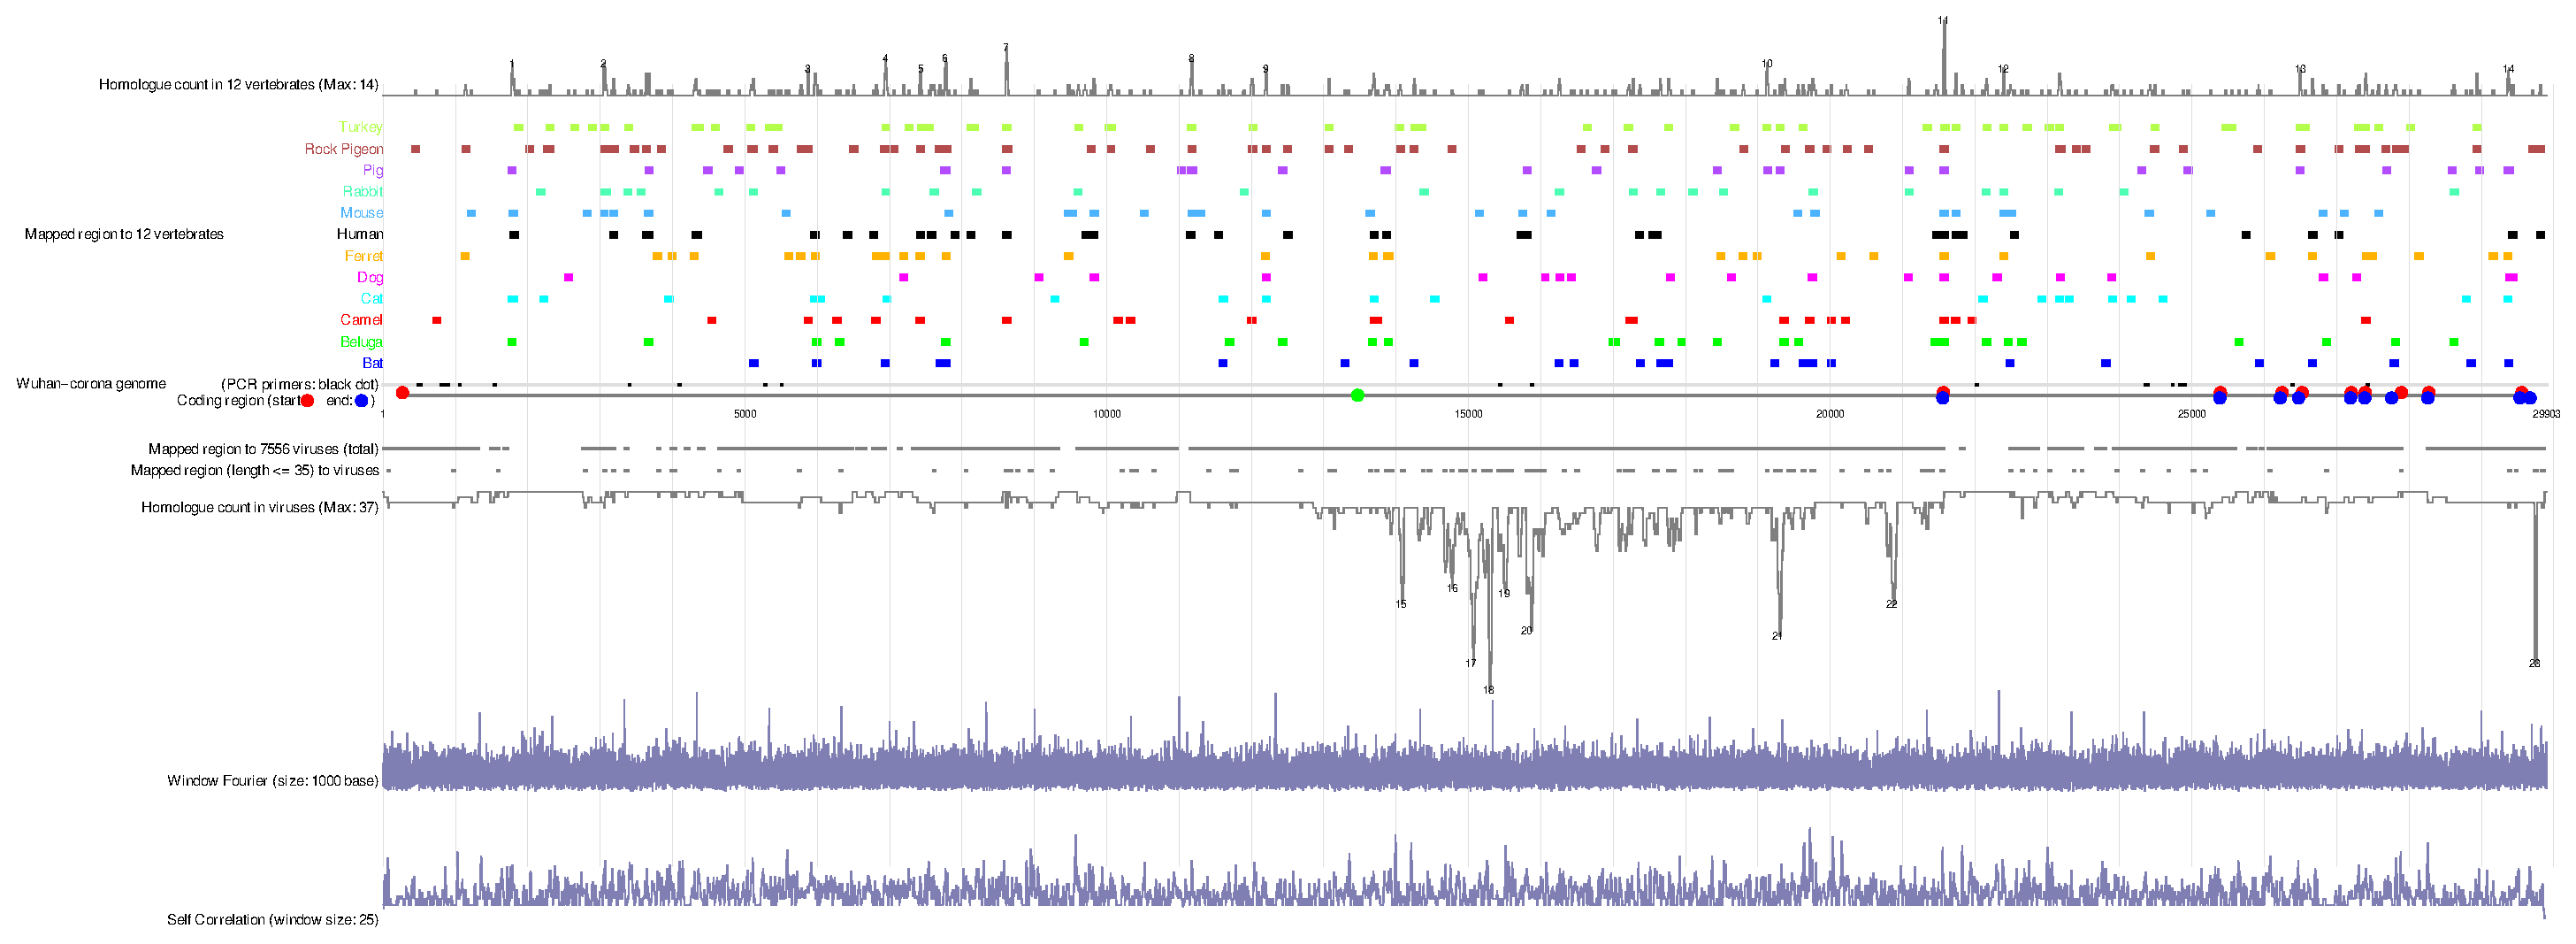
\epsfig{file=g1.eps,height=150mm}} & &  \\
 & 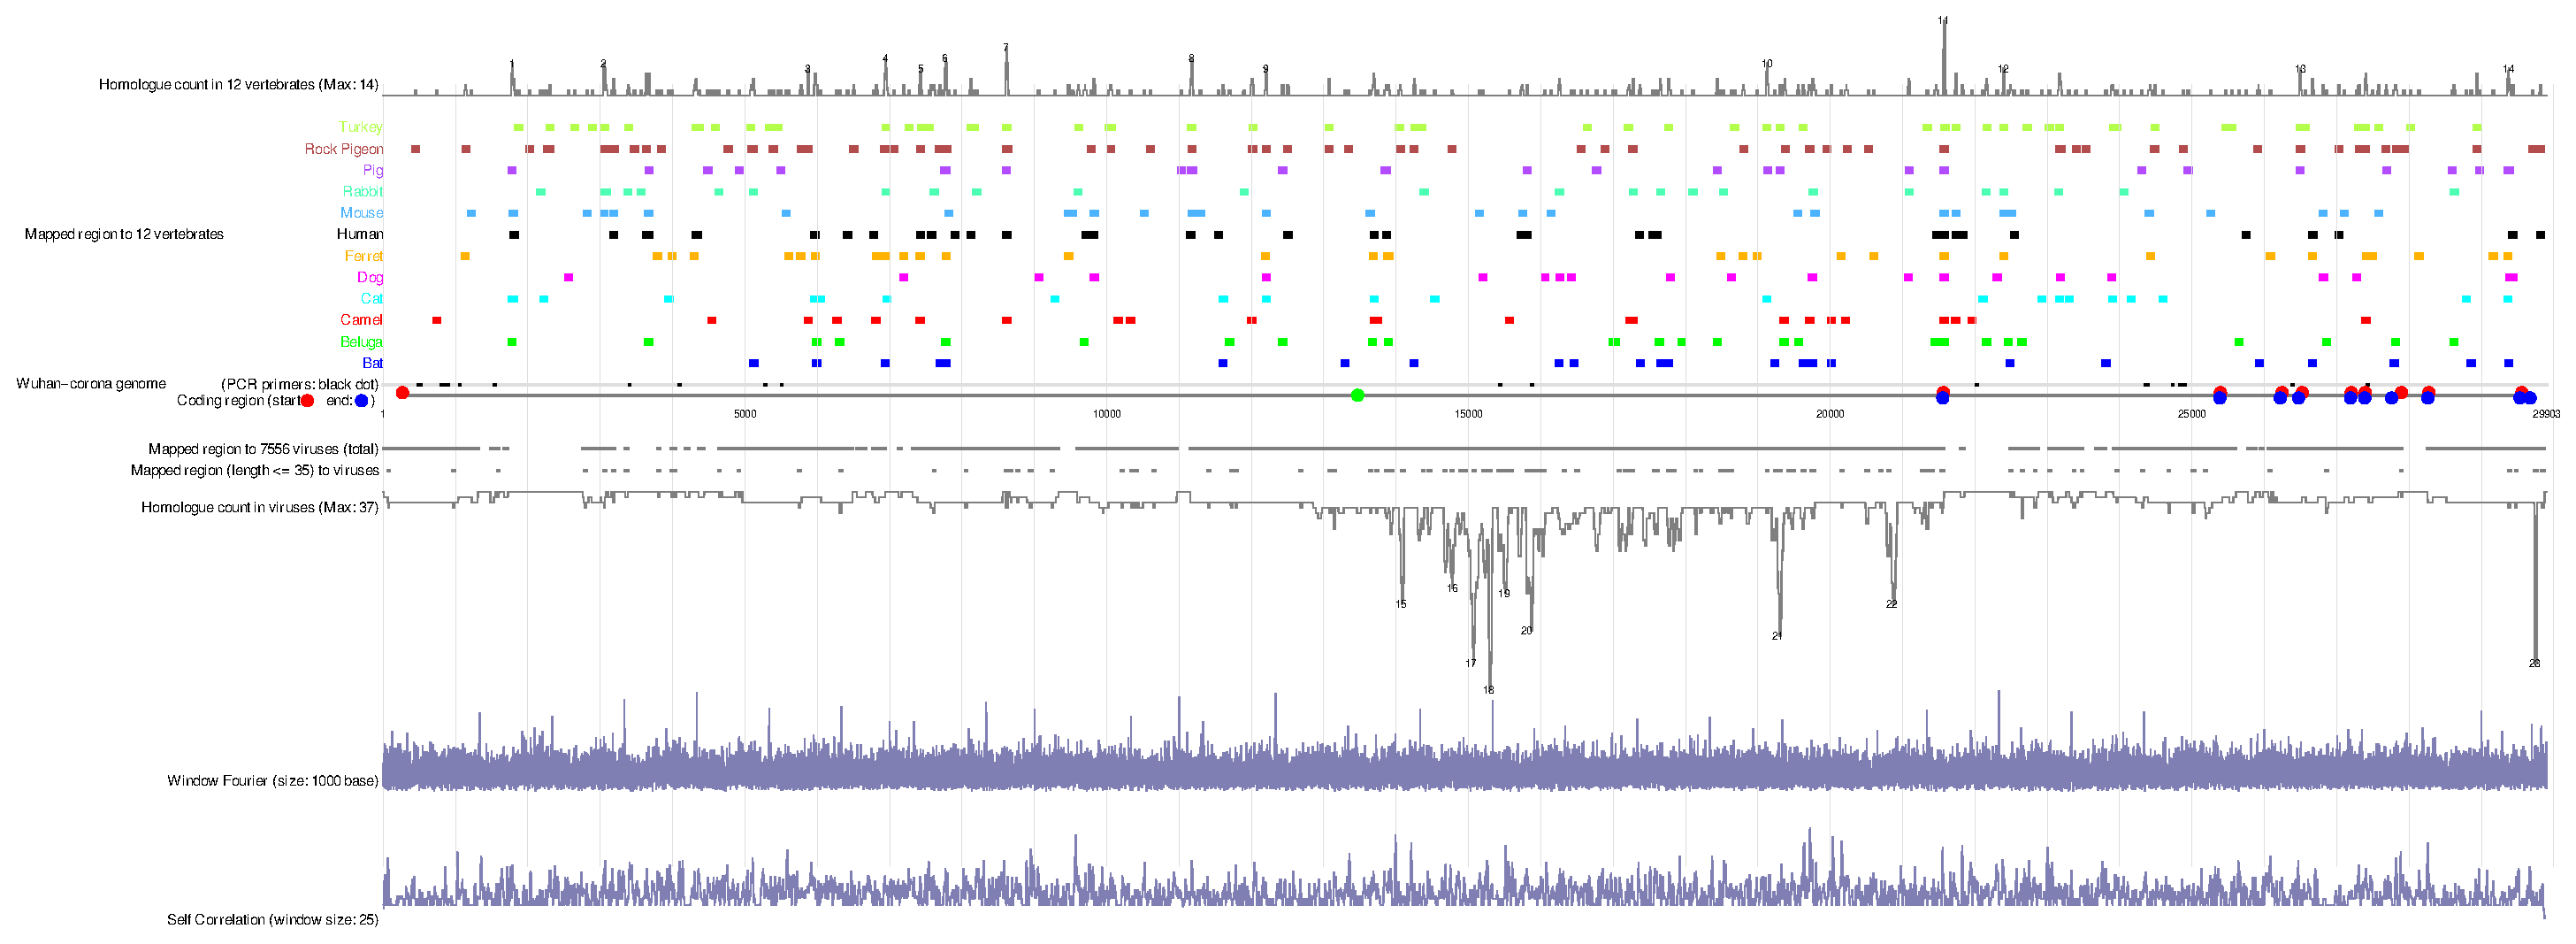
\epsfig{file=g1.eps,height=150mm} &  \\
\end{tabular}\end{center}
\color[cmyk]{1,1,0,0.8}
\end{minipage} }

\end{center}
%%----- Body, Single Column Region *) -----%%

%%----- (* Footer, Single Column Region -----%%
%\vspace{-20mm}
\color[cmyk]{0,0,0,1}
\linespread{1.0}\fontsize{22}{20}\selectfont
\begin{flushright}
References are in proceedings of the 2020 JSIMS annual meeting. \\
@ JSIMS 2020-07-04 on web meeting
\end{flushright}
%%----- Footer, Single Column Region *) -----%%



%%----- (*  Logo -----%%
%\begin{center}
%%\begin{tabular}{ccccccc}
%\begin{tabular}{ccccc}
%\epsfig{file=Tsukuba-Univ-mark200.eps,height=50mm} &
%\spaceV &
%%\epsfig{file=nias_logo.ps,height=50mm} &
%\spaceV &
%\epsfig{file=riken_g.eps,height=50mm} \\
%\end{tabular}
%\epsfig{file=KAKEN_logo.eps,height=35mm}
%\end{center}
%%-----  Logo *) -----%%


%%----- (* For print all image -----%%
%\begin{center}
%\epsfig{file=WhiteSpace.ps,height=25mm}
%\vspace{25mm}
%\end{center}
%%----- For print all image *) -----%%


\end{document}
